\documentclass[a4paper,10pt]{article}
\usepackage{float}
\usepackage{subcaption}
\usepackage{mathtools}
\usepackage{amsmath}
\usepackage{bm}
\usepackage{amsmath,amssymb}
\usepackage[algoruled,linesnumbered]{algorithm2e}
\usepackage[T1]{fontenc}
\usepackage[style=ieee]{biblatex}
\usepackage{setspace}

\usepackage{tikz}
\usepackage{tkz-euclide}
\usetkzobj{all}
\usetikzlibrary{calc}

\usepackage{geometry}
\geometry{a4paper, left=2.5cm, right=2.5cm, top=4cm, bottom=4cm}

\DeclarePairedDelimiter{\abs}{\lvert}{\rvert}
\DeclarePairedDelimiter{\norm}{\lVert}{\rVert}
\DeclarePairedDelimiter{\floor}{\lfloor}{\rfloor}

\setlength{\parskip}{1em}

\addbibresource{writeup.bib}

\begin{document}

\begin{titlepage}
  \begin{center}

  \rule{\textwidth}{1pt}\\
  \vspace{0.4cm}
  \huge
  \textbf{Real-time Watercolour using Weighted Silhouettes and Texture Generation}
  \rule{\textwidth}{1pt}\\
  \vspace{0.5cm}
  Gabrielius \v{S}lakaitis\\
  \Large
  \today
  \vfill
  
  \begin{figure}[htbp!]
    \centering
    \begin{minipage}{0.33\columnwidth}
      \includegraphics[width=\textwidth]{figures/ex1.png}
    \end{minipage}
    \begin{minipage}{0.33\columnwidth}
      \includegraphics[width=\textwidth]{figures/ex2.png}
    \end{minipage}
  \end{figure}
  \vspace{0.5cm}
  Oriel College\\
  University of Oxford\\
  Trinity 2020\\
  \end{center}
\end{titlepage}

\begin{spacing}{0}
  \tableofcontents
\end{spacing}
\newpage

\section*{Abstract}

This paper will implement a range of techniques which draw arbitrary objects as watercolour paintings in real time. It applies a geometric approach in rendering the silhouettes of the objects, which categorises the edges that need to be drawn and culls the rest. I further extend this technique to convey the lighting in the scene by dynamically varying edge weights, as well as investigate different approaches to remove edge cracking artifacts caused at the intersections of thick lines. I also devise a texture generation method that provides a watercolour fill. Its idea is to generate a set of points tied to the surface of the mesh which act as anchors for texture generation. These points move naturally in the 3D scene and provide the desired temporal coherence when moving around the objects, but the 2D screen coordinates of these points can be used as parameters for the watercolour effect. Finally, I apply screen-space effects to give the illusion that the whole scene is on paper, completing the overall effect.

%%%%%%%%%%%%%%%%%%%%%%%%%%%%%%%%%%%%%%%%

\section{Introduction}

Often in industry the success of graphics software is measured by how close it mimics reality. It is frequently assumed that this increases immersion in games or makes applications more professional. However this is not always the case; commonly, using non-photorealistic techniques allows for graphical aspects of a program to be tailored to improve the overall product. In design applications, outlines and special shading methods might be used to improve clarity \cite{Gooch1998}. In games and animations, a certain rendering style might help the user experience certain emotions sought by the creators. In addition, non-photorealistic methods largely require lower computational power to run, as well as reduce development times and costs. Inspired by the benefits, I have decided to produce a renderer which takes 3D scenes as inputs and produces watercolour renderings.

There are many watercolour techniques artists use to produce various styles of work. In the one simulated here, watercolour is used in combination with ink: the outlines of objects are traced in a dark colour to provide the basis for the shapes, and then each one is shaded in a block colour. This is simplistic and does not provide every detail of the object, as this is not the ultimate goal; observing any artwork is largely an interpretive process. To communicate lighting while still having block colours, the silhouette lines will vary in weight so that the darkest regions appear bolder.
%* this paragraph was a bit of a mess?

The first stage is the outlining. Most of the methods for silhouette shading are image-based and rely on feature extraction from buffers - where discontinuities in the depth buffer correspond to silhouettes \cite{Saito1990}. While this works for most applications, it would be difficult to flexibly vary the line width using this method, as each fragment does not know how close it is to a given edge. A different approach solves these issues by lighting an object from the point of the camera, which leads to fragments near the silhouette being the darkest. A threshold can then be applied to draw the outline. A composition between this headlight and scene lighting can also be used to communicate particular illumination. The problem with this method, and similar advanced techniques \cite{Goodwin2007}, is that they require smooth model surfaces, whereas the goal of this paper is to present a solution for arbitrary objects.

Geometric methods are also used to render silhouettes. A common approach is the use of a stencil buffer. The object writes some constant value to the buffer when rendered, and then the same object is drawn in thick wireframe wherever the stencil value was not set, giving the desired outline \cite{McGuire2004}. The disadvantage of this method is that any silhouette that is seen on the body of the object will not be visible, stripping all detail from it. To concisely distinguish all silhouette features, a property is devised. An edge is on the silhouette if one of its neighbouring faces is front-facing, and the other is back-facing. All edges not satisfying this property will be culled without wasting performance in rasterisation, and the geometric approach will provide flexibility to alter the edge weights as necessary. However, making the CPU characterize these edges every frame, and passing the correct ones for the GPU to render would quickly become a bottleneck. This problem is tackled by passing adjacent face information about every edge to the GPU, where it can check this property in parallel \cite{Hughes2004}. In this paper I extend this basic idea, and use the edge information to calculate unique lighting properties of the silhouette edges, achieving the desired effect.

The second stage will apply a watercolour texture and shade to the objects. A common technique for non-photorealistic rendering is cel shading, where light intensity thresholding is applied to the regularly shaded object, creating fields of different light intensities. While this is a great effect for cartoons and some drawings, sharp field edges and small areas of shading can look unnatural, so it will be avoided from this simplistic approach where the lighting is already implied by the weight of the edge. All objects will be drawn in solid colours with a watercolour effect.

Granulation and flocculation of watercolour pigments \cite{Curtis1997} can be roughly simulated by applying some noise and a paper texture to the object fill. However, the application of such textures often leads to continuity issues. Trivially, the texture could be applied to the meshes themselves, but this is not satisfactory - the result will not give the illusion of 2D paint, since viewing faces at an angle will compress these textures. A simple method to generate a flat image takes a watercolour texture spanning the whole screen and crops it to match the shape of the object. While this looks satisfactory for stills, moving around the object is unnatural - as if the object was a hole through which the texture is seen. This can be solved for vertical and horizontal movement, as well as movement towards and away from an object by translating and scaling the texture. Rotation, however, has no trivial solution.
%* last sentence?

Several methods successfully tackle similar issues. In one, textures and details are annotated by an artist as strokes with different properties \cite{Kalnins2002}. Such strokes form a base path, on which a triangle strip can be rendered with the selected texture. The obvious downside of this is that an artist has to provide such details; the rendering method cannot be used on a plain mesh. In addition, it is difficult to generate whole areas of colour using just strokes. Another method generates a texture from a given paint sample by an image quilting algorithm \cite{Kulla1989}. It cuts random blocks out from the sample and pastes them to the target image, ensuring optimal overlap boundaries between the squares for smooth transitions. For temporal coherence, it tries to match the current frame as closely as possible to the previous, however this does not completely smooth out the shower door effect (and leads to lack of consistency in the location of particular details of the objects). The approach outlined in this paper tackles the problem by generating a set of key points on the 3D mesh, which act as anchor points for the texture. These points behave naturally when moving around an object as they are attached to the surface, and the screen coordinates of these anchor-points can be used as parameters in the generation of a 2D texture. Many effects could be produced with these parameters, but in this paper I will consider a simple version which places a 2D brush-texture on each one of the anchor-points in the target image. This will provide perfect temporal coherence as well as the illusion of a flat watercolour texture.

The full contributions of this paper therefore include several implementations of real-time methods as follows. First is geometric silhouette detection, which gives the objects outlines and details by characterising the edges to be drawn and removing the rest. I describe what necessary mesh information is needed and how it is used to draw lines of desired width in real-time by the shaders. Variations of the method are executed to highlight advantages in using alternative line joining methods. In addition, a separate rendering pass is used to hide edges that are covered by the object; employing the depth buffer and the original mesh to draw over these silhouettes. Second is a texture generation technique that I have designed with temporal coherence in mind. A solid colour will be used to fill the whole mesh and given brush textures will be applied to screenspace anchor-points pinned to the surface of the mesh - cropping any textures that bleed outside of the object fill. I detail how the anchor-points are generated in preprocessing, as well as how their information is used to render the textures and ensure coherence by calculating their visibility in the shaders. I further analyse the method and introduce solutions that deal with any effects that may be considered unsatisfactory. Lastly, buffer objects are used to render the scene into memory and apply several screen-space effects. One of them is wobbling, which simulates bleeding of paint by using a paper texture - a fragment may use the colour of one of its neighbours, making even lines appear rough. Another is the use of a paper bump map to make it appear like the whole scene is drawn on paper, which also interacts real-time with the lighting of the scene.


%%%%%%%%%%%%%%%%%%%%%%%%%%%%%%%%%%%%%%%%

\section{Silhouette Shading}

The technique of silhouette shading aims to achieve two effects. The first is to set a boundary between the area that is shaded and the blank page, highlighting details that may be hard to spot due to the two-dimensionality of the image. The second is to provide a communication of lighting - render bold lines in the shadowed sections of the silhouette and thin lines in the light. This will not only provide some necessary information about the scene, but also give the illusion of an artist's touch due to the varying line weights.

In summary, this method will only render the edges that are on the silhouette of the object, defined by one neighbouring face being turned towards the camera and the other being turned away. The test of whether this is true will be computed in the vertex shader, and the edges not satisfying this property will be disregarded. For this test to be run, the shader will require access to the face normals adjacent to the considered edge, which will be computed in the preprocessing step and passed in. If an edge does have to be drawn, its weight will be determined by comparing the direction of the edge normal and the light.

In this paper the scene lighting will consist of one point source, however this mechanism can be modified arbitrarily, and the lighting can change over time.

\subsection{Preprocessing}
In order to pass the required information to the GPU, a list of edges needs to be constructed. Neighbouring face normals and vertex normals should also be known for each edge. However, most generic mesh formats only store a list of the coordinates of each vertex, followed by a list of faces represented as groups of these vertices. It is also a convention for every face to have its own version of a vertex for texturing purposes, which leads to a single corner of a model often having three or more vertices associated with it. This is a problem since the vertex normals cannot be calculated by averaging the normals of faces that include it, and finding unique edges becomes a challenge. This preprocessing step will extract this necessary information from any given mesh before any rendering is done.

In all standard formats we can easily iterate through the faces of the model and access each of the vertices associated with it. For uniqueness, this step stores discovered vertices only by their coordinates, and edges by the coordinates of their end-vertices in lexical order. To calculate the vertex normals, one unordered map structure keeps key-value pairs with vertices as keys and their accumulating normals as values. If a new vertex is discovered while iterating through the faces, a new pair is added storing the vertex and the current face normal. If the vertex is already in the map, then the current face normal is added to the value at the pair. Clearly after every face is visited, this map will contain the sum of adjacent face normals for every vertex, which can be normalized to get the vertex normal. For adjacent faces, a second unordered map contains edges and one of their neighbouring face normals as the key-value pairs. If a new edge is discovered, then a pair of the edge and the current face normal is added to the map. If an edge is already there, then both its neighbouring face normals can be accessed and stored, since an edge can only have at most two neighbours. By the end of this process all edges and their neighbouring faces can be accessed, and the vertex normals looked up via the first map.

Even if this stage only happens once at the start of the program, a very large number of vertices may be processed, so an unordered map structure is used to reduce the loading time. This means writing and accessing of elements are $O(1)$ operations, making the whole preprocessing stage run in $O(\abs{faces})$ time. In practice this happens almost instantly for a few thousands faces, but slows as a million or more are approached.


\subsection{Rendering the edge}
Using line primitives to draw the silhouette in OpenGL leads to uncertainty. In some cases using a particular line width might not be supported by an implementation and if this happens, the closest supported width would be used. In fact most graphics APIs do not guarantee the ability to rasterize lines of any width other than one pixel. This means constructing the edges from triangles is the only reliable option as the exact dimensions can be accurately controlled. In addition, line joining is not supported, which leads to artifacts as shown in Figure \ref{cap} when drawing thick lines, which can also be fixed using triangles. There are several styles of line joins that could be used to add caps between two lines \cite{Drakos1999}. However, they all rely on some knowledge about both edges, and the GPU will not have this information since processing is independent. To counter this problem I will modify and extend an algorithm published in a paper by McGuire and Hughes \cite{Hughes2004}, that uses the vertex normal - which falls between the two quads in the crack - to generate the edge caps. This is the only mutual information available between edges.

\begin{figure}[htbp!]
  \centering
  \begin{subfigure}{0.2\columnwidth}
    \includegraphics[width=\textwidth]{figures/1_1.png}
  \end{subfigure}
  \begin{subfigure}{0.2\columnwidth}
    \includegraphics[width=\textwidth]{figures/1_2.png}
  \end{subfigure}
  \caption{Edge caps fix cracks caused by bold lines.}
  \label{cap}
\end{figure}

Six points are required in order to draw an edge from triangles. The first four points form the main quad: with two points at the base of the line and the other two extruding perpendicular to the direction of the line (to retain the negative space of the object no matter the width of the line, the silhouette of the object should be drawn on the exterior). The last two points are used in order to draw the caps on either side and extend along the direction of the vertex normal. Since any two adjacent edges will share this vertex and its normal, this will be a common point between them, so long as they are extended by the same amount. In any of these cases the magnitude of extrusion will depend on the lighting calculations.

The required attributes for every vertex passed into the shader are ($v$, $v'$, $n$, $n_A$, $n_B$, $i$) where $v$, $v'$ are the vertices at the base of the edge; $n$ is the vertex normal; $n_A$, $n_B$ are the adjacent face normals and $i$ is an integer between 0 and 2 determining whether this vertex represents the base, the roof or the cap of the edge. Note that $i$ only represents the type of the vertex, whereas which end of the edge it will be on is determined by the $v$ and the corresponding $n$.

\begin{figure}[htbp!]
  \centering
  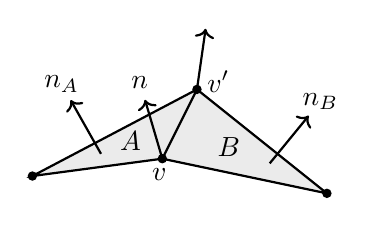
\begin{tikzpicture}
    \def\size{0.06}
    \coordinate (A) at ( 0.0, 0.0);
    \coordinate (B) at ( 0.44, 0.88);
    \coordinate (C) at (-1.65,-0.22);
    \coordinate (D) at ( 2.09,-0.44);
    \coordinate (NV)  at (-0.22, 0.748);
    \coordinate (NV') at ( 0.11, 0.77);
    \coordinate (NA)  at (-0.385, 0.682);
    \coordinate (NB)  at ( 0.495, 0.605);
    \fill[color=black!8!white] (A) -- (C) -- (B) -- (D);
    \fill[color=black] (A) circle (\size); \fill[color=black] (B) circle (\size); \fill[color=black] (C) circle (\size); \fill[color=black] (D) circle (\size);
    \draw[thick] (A) node[anchor=80]{$v$} -- (B) node[anchor=-160]{$v'$} -- (C) -- (A) -- (D) -- (B);
    \draw[thick,->] (A) -- ($(A)+(NV)$) node[pos=1.3]{$n$};
    \draw[thick,->] (B) -- ($(B)+(NV')$);%node[anchor=-110]{$n_B$};
    \draw[thick,->] ($0.38*(B)+0.62*(C)-0.2*(NA)$) -- ($0.38*(B)+0.62*(C)+0.8*(NA)$) node[pos=1.3]{$n_A$};
    \draw[thick,->] ($0.38*(B)+0.62*(D)-0.2*(NB)$) -- ($0.38*(B)+0.62*(D)+0.8*(NB)$) node[pos=1.3]{$n_B$};
    \node at ($1/3*(A)+1/3*(B)+1/3*(C)$) {$A$};
    \node at ($1/3*(A)+1/3*(B)+1/3*(D)$) {$B$};
  \end{tikzpicture}
  \caption{Attributes of the edge.}
  \label{info}
\end{figure}

The first thing that the shader has to work out is the weight of the line. In conventional shading the lighting is calculated by using the face normal: the further away from the light a face is, the darker it will be drawn. For edges, it is natural to take the average of the face normals that it lies between - the edge normal - and use this for the lighting. Then the standard calculation is applied: $w = light \cdot normal$. Parameters can be used to take this value from [-1, 1] to the desired range.

Each one of the six vertices passed into the shader will represent a point of the edge depending on their kind $i$. The first step of the shader is to calculate the screen coordinates of  $v$, $v'$ and the vector $n$. These will be represented as $s$, $s'$ and $m$. If the type of the vertex is the base of the edge ($i=0$), then the final position is simply $s$. Otherwise the shader calculates the line direction vector $s'-s$, and its perpendicular - $p$, found by swapping the x and y coordinates of the direction vector and then negating the x coordinate. To ensure the quad extrudes away from the surface of the mesh, check that the direction of the edge normal (screen space version of $n_A+n_B$) and this perpendicular vector point in the same direction. If it is not the case, negate $p$. Then normalize it and multiply it by the weight of the line $w$ to make its length $w$. If the type of the vertex is the roof ($i=1$), then the final position is $s+p$. Finally, if the vertex is the cap ($i=2$), the vector $m$ is lengthened to $w'$ in a similar fashion and the final position becomes $s+v$. Note that we cannot use $w$ to extend the cap vertex, since this value will be different for the two joining edges. A mutual weight is calculated using the vertex normal rather than the edge normal to create a smooth transition, which will have a magnitude in the middle of the two edge weights.

\begin{figure}[htbp!]
  \centering
  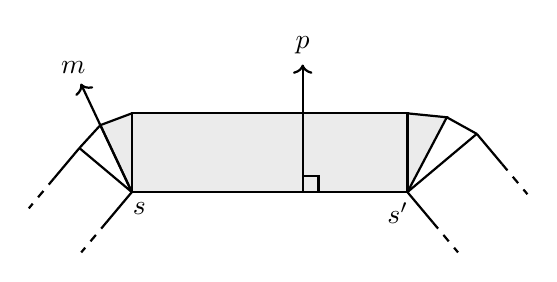
\begin{tikzpicture}
    %line info
    \def\len{3.5}
    \def\theta{50}
    \def\w{1}
    \def\ratio{1.15}
    \def\clenl{0.5}
    \def\clenr{0.5}
    \def\right{0.2}
    %cap points
    \coordinate (C)  at (-0.4,\w-0.15);
    \coordinate (C') at (\len+0.5,\w-0.05);
    %coordinates
    \coordinate (B)  at (0,0);
    \coordinate (R)  at (0,\w);
    \coordinate (B') at (\len,0);
    \coordinate (R') at (\len,\w);
    \coordinate (N)  at ({-\w/\ratio*sin(\theta)},{\w/\ratio*cos(\theta)});
    \coordinate (N') at ({\len+\w*\ratio*sin(\theta)},{\w*\ratio*cos(\theta)});
    %fill
    \fill[color=black!8!white] (B)  rectangle (R');
    \fill[color=black!8!white] (R)  -- (C)  -- (B);
    \fill[color=black!8!white] (R') -- (C') -- (B');
    %draw edges
    \draw[thick] (B)  rectangle (R');
    \draw[thick] (B)  -- (N);
    \draw[thick] (B') -- (N');
    \foreach \x/\y in {0/0,{-\w/\ratio*sin(\theta)}/{\w/\ratio*cos(\theta)}}{
        \draw[thick] ({\x},{\y}) -- ({\x-\clenl*cos(\theta)},{\y-\clenl*sin(\theta)});
        \draw[thick,dashed] ({\x-\clenl*cos(\theta)},{\y-\clenl*sin(\theta)}) -- ({\x-\clenl*2*cos(\theta)},{\y-\clenl*2*sin(\theta)});}
    \foreach \x/\y in {\len/0,{\len+\w*\ratio*sin(\theta)}/{\w*\ratio*cos(\theta)}}{
        \draw[thick] ({\x},{\y}) -- ({\x+\clenr*cos(\theta)},{\y-\clenr*sin(\theta)});
        \draw[thick,dashed] ({\x+\clenr*cos(\theta)},{\y-\clenr*sin(\theta)}) -- ({\x+\clenr*2*cos(\theta)},{\y-\clenr*2*sin(\theta)});}
    \draw[thick] (R)  -- (C)  -- (B)  node[anchor=90+\theta/2]{$s$};
    \draw[thick] (R') -- (C') -- (B') node[anchor=90-\theta/2]{$s'$};
    \draw[thick] (N)  -- (C);
    \draw[thick] (N') -- (C');
    %draw arrows
    \draw[thick,->] ({0.62*\len},0) -- ({0.62*\len},{1.62*\w}) node[anchor=south]{$p$};
    \draw[thick] ({0.62*\len},\right) -- ({0.62*\len+\right},\right) -- ({0.62*\len+\right},0);
    \draw[thick,->] (B) -- ($(B)+1.62*(C)$) node[anchor=-90+\theta/2]{$m$};
  \end{tikzpicture}
  \caption{Rendering the edge and its corresponding caps.}
\end{figure}

One slightly tedious consideration concerns the fact that the screen coordinates range from -1 to 1 for both x and y coordinates, no matter the aspect ratio. The ratio itself is therefore also passed into the shader and the screen coordinates are modified accordingly.

The vertices describing every edge will be passed into the vertex shader as one long list - every six vertices defining one edge. On top of that, information has to be given about where to draw the triangles between such vertices. This is in the form of an index list, where every three indices represent a triangle that should be rendered. For each edge $e$ (which has respective vertices ranging from 6$e$ to 6$e$+5) a 12 index list section is defined that describes these four triangles: [6$e$, 6$e$+2, 6$e$+3, 6$e$, 6$e$+3, 6$e$+1, 6$e$, 6$e$+4, 6$e$+2, 6$e$+1, 6$e$+3, 6$e$+5]. This pattern is repeated for every $e$.

Of course, edges should only be visible if they are on the silhouette of the shape. This is characterized by the case where only a single one of the faces can be seen from the eye position. Formally this is represented as the following formula:
$$[n_A \cdot (eye-v) < 0] \oplus [n_B \cdot (eye-v) < 0]$$
Note that it does not matter whether $v$ or $v'$ are used in this formula, so this will not cause an issue where only one side of the edge is clipped. If this constraint is not satisfied by the attributes of a vertex, it means that they represent an edge which shouldn't be seen. Unfortunately the vertex shader is unable to directly destroy such geometry, but its position can be changed. In particular, the vertices of such an edge will be transformed behind the clipping plane. Simply put, we are taking all the edges that shouldn't be seen and moving them behind the camera, where they will be discarded. Since clipping happens before rasterisation in the graphics pipeline, these vertices will be discarded early and not cost much processing power.


\subsection{Alternative solutions}
The algorithm for construction edges and caps in the given way is not perfect in all scenarios. All edges have a constant width from one side to the other. This is exactly what is required when drawing low-poly objects where straight lines do in fact represent a flat surface, but not always satisfactory when trying to represent a smooth curve.

\paragraph{Vertex-based weights.}
This is a direct translation of the Gouraud shading method, which is usually used to render faces by calculating the colour at each vertex and interpolating across. Similarly, this alternate method uses the weight value calculated using the vertex normals and extending each side of the edge accordingly. The result is shown in Figure \ref{smooth}.

\begin{figure}[htbp!]
  \centering
  \begin{subfigure}{0.25\columnwidth}
    \includegraphics[width=\textwidth]{figures/2_1f.png}
    \caption{Regular}
  \end{subfigure}
  \begin{subfigure}{0.25\columnwidth}
    \includegraphics[width=\textwidth]{figures/2_2f.png}
    \caption{Vertex-based}
  \end{subfigure}
  \caption{Avoiding steps using an alternative weight method.}
  \label{smooth}
\end{figure}


This approach leads to an easy optimisation. Since in this method the cap vertex and the roof vertex extend from the base by the same amount we can completely get rid of the roof vertices and  construct the whole edge out of just the four points. Understandably, due to the fact that the vector $m$ is not perpendicular to the edge, the width of the line will decrease. In practice this is not a problem - especially since this method will be used when the shape is smooth, and the angle between $n$ and $p$ low.

\begin{figure}[htbp!]
  \centering
  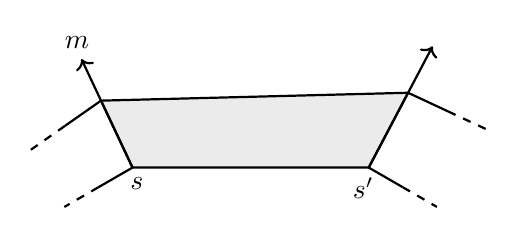
\begin{tikzpicture}
    %line info
    \def\len{3}
    \def\theta{30}
    \def\w{1}
    \def\ratio{1.15}
    \def\clenl{0.5}
    \def\clenr{0.5}
    \def\right{0.2}
    %cap points
    \coordinate (C)  at (-0.4,\w-0.15);
    \coordinate (C') at (\len+0.5,\w-0.05);
    %coordinates
    \coordinate (B)  at (0,0);
    \coordinate (B') at (\len,0);
    \coordinate (N)  at ({-\w/\ratio*sin(\theta)},{\w/\ratio*cos(\theta)});
    \coordinate (N') at ({\len+\w*\ratio*sin(\theta)},{\w*\ratio*cos(\theta)});
    %fill
    \fill[color=black!8!white] (B) -- (C) -- (C') -- (B') -- cycle;
    %draw edges
    \draw[thick] (B) node[anchor=90+\theta/2]{$s$} -- (C) -- (C') -- (B') node[anchor=90-\theta/2]{$s'$} -- cycle;
    \foreach \x/\y [count = \i] in {0/0,{-0.4}/{\w-0.15}}{
        \def\ttheta{\theta+(\i-1)*5}
        \def\tlen{(\clenl+(\i-1)*0.06)}
        \draw[thick] ({\x},{\y}) -- ({\x-\tlen*cos(\ttheta)},{\y-\tlen*sin(\ttheta)});
        \draw[thick,dashed] ({\x-\tlen*cos(\ttheta)},{\y-\tlen*sin(\ttheta)}) -- ({\x-\tlen*2*cos(\ttheta)},{\y-\tlen*2*sin(\ttheta)});}
    \foreach \x/\y [count = \i] in {\len/0,{\len+0.5}/{\w-0.05}}{
        \def\ttheta{\theta-(\i-1)*5}
        \def\tlen{(\clenr+(\i-1)*0.06)}
        \draw[thick] ({\x},{\y}) -- ({\x+\tlen*cos(\ttheta)},{\y-\tlen*sin(\ttheta)});
        \draw[thick,dashed] ({\x+\tlen*cos(\ttheta)},{\y-\tlen*sin(\ttheta)}) -- ({\x+\tlen*2*cos(\ttheta)},{\y-\tlen*2*sin(\ttheta)});}
    %draw arrows
    \draw[thick,->] (B)  -- ($(B)+1.62*(C)$) node[anchor=-90+\theta/2]{$m$};
    \draw[thick,->] (B') -- ($1.62*(C')-0.62*(B')$);
  \end{tikzpicture}
  \caption{Rendering an edge using vertex-based weights.}
\end{figure}


While this is a great improvement, there is still an issue present in this result relating to smooth surfaces. Each edge or vertex has some weight value, depending on its direction to the light. The result of edge culling means that we can only see an edge if it's on the very silhouette of the mesh. At some point in time while rotating around an object, the current edge on the silhouette would be completely hidden behind a face, and a new edge would emerge as the silhouette. Since this edge would have a distinct weight to the previous one, there would be a point in time when the silhouette jumps from the width of the first to the second. Clearly this is an issue for both methods. This artifact is also seen in still images when there's added curvature in the mesh, as in Figure \ref{turn}. At certain points a sudden switch occurs between the light value of the edges on this curved mesh. The artifact strongly depends on the model shape, how its lines are organised, the point of view and the position of the light, but it still breaks continuity in some cases. Once again, this could be the desired effect when considering low-poly objects, but not when we want something to appear smooth. 

\begin{figure}[htbp!]
  \centering
  \begin{subfigure}{0.25\columnwidth}
    \includegraphics[width=\textwidth]{figures/3_1.png}
    \caption{Regular}
  \end{subfigure}
  \begin{subfigure}{0.25\columnwidth}
    \includegraphics[width=\textwidth]{figures/3_2.png}
    \caption{Vertex-based}
  \end{subfigure}
  \begin{subfigure}{0.25\columnwidth}
    \includegraphics[width=\textwidth]{figures/3_3.png}
    \caption{Tangent-based}
  \end{subfigure}
  \caption{Artifact due to edge-dependent calculations.}
  \label{turn}
\end{figure}

\paragraph{Tangent-based weights.}
In order to make the edges independent from their weight, edge normals or vertex normals cannot be used for the lighting calculation. Instead, the position of the eye in relation to the edge proves to be helpful. The vector describing the gaze from the eye to a particular point of the mesh can be easily found. Imagining the surface of the mesh to be infinitely smooth, no matter the position of the eye, the normal vector on the silhouette will be exactly perpendicular to the this gaze, as in Figure \ref{gaze}. To fully define this normal in three dimensions it needs another parameter. The direction of the edge itself can be used for this, since the normal has to be perpendicular to this edge. Now this normal can be expressed formally:
$$(v-eye) \times (v-v_2)$$

\begin{figure}[htbp!]
  \centering
  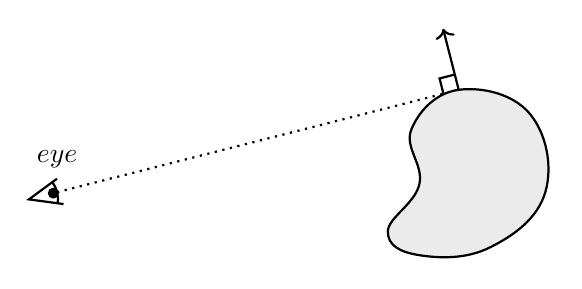
\begin{tikzpicture}
    \pgfmathsetmacro{\arrowlen}{0.8}
    \pgfmathsetmacro{\right}{0.2}
    \pgfmathsetmacro{\eyeX}{-5.1}
    \pgfmathsetmacro{\eyeY}{-1.3}
    \def\len{sqrt(\eyeX*\eyeX+\eyeY*\eyeY)}
    \coordinate (E) at (\eyeX, \eyeY);
    \coordinate (OE) at ({\eyeX/\len},{\eyeY/\len});
    \coordinate (OP) at ({\eyeY/\len}, {-\eyeX/\len});
    \draw[thick,dotted] (E) -- (0,0);
    \draw[thick,->] (0,0) -- ($\arrowlen*(OP)$);
    \draw[thick] ($\right*(OE)$) -- ($\right*(OE)+\right*(OP)$) -- ($\right*(OP)$);
    \fill[color=black!8!white] plot[smooth cycle,tension=0.7] coordinates {(0,0) (0.9,-0.3) (1.1,-1.3) (0.4,-2) (-0.5,-2.1) (-0.9,-1.8) (-0.5,-1.2) (-0.6,-0.5)};
    \draw[thick] plot[smooth cycle,tension=0.7] coordinates {(0,0) (0.9,-0.3) (1.1,-1.3) (0.4,-2) (-0.5,-2.1) (-0.9,-1.8) (-0.5,-1.2) (-0.6,-0.5)};
    %\fill[color=black!8!white] plot[smooth cycle,tension=0.7] coordinates {(0,0) (0.63,-0.21) (0.77,-0.91) (0.28,-1.4) (-0.35,-1.47) (-0.63,-1.26) (-0.35,-0.84) (-0.42,-0.35)};
    %\draw[thick] plot[smooth cycle,tension=0.7] coordinates {(0,0) (0.63,-0.21) (0.77,-0.91) (0.28,-1.4) (-0.35,-1.47) (-0.63,-1.26) (-0.35,-0.84) (-0.42,-0.35)};
    \pgfmathsetmacro{\eye}{0.37}
    \pgfmathsetmacro{\width}{22}
    \def\angle{atan(\eyeY/\eyeX)}
    \coordinate (B) at ($(E)+\eye*(OE)$);
    \coordinate (L) at ({cos(\angle-\width)},{sin(\angle-\width)});
    \coordinate (U) at ({cos(\angle+\width)},{sin(\angle+\width)});
    \draw[thick] ($(B)+1.2*\eye*(L)$) -- (B) -- ($(B)+1.2*\eye*(U)$) node[anchor=-90]{$eye$};
    \draw[thick] (E) arc (\angle:\angle+\width:\eye);
    \draw[thick] (E) arc (\angle:\angle-\width:\eye);
    \fill[color=black] ($(E)+0.05*(OE)$) circle (0.07);
  \end{tikzpicture}
  \caption{The normal is perpendicular to the tangent from the eye in smooth shapes.}
  \label{gaze}
\end{figure}


The artifact is indeed solved (and there is an added benefit that the vertex normal is not needed as a parameter). However, The use of edge direction means that edges have a uniform weight throughout once again - leading to the same steps on the curve as in the original method. Sadly this problem is not easily fixed. It would be intuitive to use the vertex normals for the second parameter to the perpendicular, instead of the direction of the edge. In fact, the calculation for the vector would then become:
$$(v-eye) \times [n \times (v-eye)]$$
rewritten to reduce shader computation as:
$$[(v-eye) \cdot (v-eye)]n - [(v-eye) \cdot v](v-eye)$$
Of course, here the dependency on the vertex normals is brought back and the original artifact reappears, rendering the intuition invalid. Although, this is a satisfactory mutual weight to use for the caps between each edge.

\paragraph{Hybrid weights.}
In reality a single object might contain one section which has sharp corners and another which is simulating a smooth surface. In this case an additional parameter can be passed that determines the type of shading that should be applied. Since this parameter would be on a per-vertex basis, the transition between these types would be smooth.\\

Between the vertex-based and tangent-based methods, both would eventually lead to perfect transitioning as the detail of the mesh tends towards infinite, but in practice the artifact caused by the vertex-based method is much less frequent. Generally the constraint of independence between edges makes the task of making the silhouette appear completely smooth a challenge - knowledge of all neighbouring edge directions and a variation of the tangent method would allow perfectly smooth transitioning in all cases.


\subsection{Covered edges}
Some of the edges that are seen using this silhouette method lay on the opposite side of the mesh to the eye. These edges should not be visible as they give away detail that is hidden by the object itself, yet they satisfy the specification of one normal facing towards and the other facing away from the position of the eye. In addition, if several objects are rendered like this, they will not obstruct each other and appear see-through. While sometimes this might be a nice effect, often it leads to uncertainty in which part of the scene is closer, and even the direction an object is facing. The technique published by Rossignac and von Emmerik \cite{Rossignac1992} will be employed in order to hide these unwanted edges by using the depth buffer (sometimes also called z-buffer).
%* z-buffer necessary?
%* strange citing, maybe throughout?

When a primitive is rendered to the screen, the depth buffer stores how far each fragment is from the screen. The further away, the higher the value. This includes the silhouette edges, since their depth values are kept when the screen coordinates are calculated. A first pass in the shader renders all of the faces of the object before the silhouette as seen in Figure \ref{cover}a. During the pass, the depth buffer values are set accordingly for each fragment. Now when the silhouette as in \ref{cover}b is drawn in a second pass, a depth test is applied. Silhouette edges that are behind an object will have a higher depth value than the one stored by the previous pass, and will not be rendered, leading to the result shown in \ref{cover}c.

\begin{figure}[htbp!]
  \centering
  \begin{subfigure}{0.3\columnwidth}
    \includegraphics[width=\textwidth]{figures/4_2.png}
    \caption{Only faces}
  \end{subfigure}%
  $\bm{+}$%
  \begin{subfigure}{0.3\columnwidth}
    \includegraphics[width=\textwidth]{figures/4_1.png}
    \caption{Only edges}
  \end{subfigure}%
  $\bm{\longrightarrow}$%
  \begin{subfigure}{0.3\columnwidth}
    \includegraphics[width=\textwidth]{figures/4_3.png}
    \caption{Combined}
  \end{subfigure}
  \caption{Two passes hide covered edges using the depth buffer.}
  \label{cover}
\end{figure}


In the original article \cite{Rossignac1992}, the z values of the lines have to be displaced forward by some amount to make sure that they are not hidden by the surrounding mesh. In this case that is not a problem, as we are only drawing the silhouette on the exterior of the object and it would never be covered by the mesh itself. This is an advantage as it avoids any artifacts caused by setting the z displacement to a value too low or high (which is non-trivial, since the optimal differs from scene to scene).

As seen in the result, this has a positive side-effect of giving some colour to an object, as well as clearly defining the region on the screen within which the object exists. Both of these facts will prove useful in the following sections.


\subsection{Comments}
Using the geometric method allows us to cull unwanted edges and process their parameters in order to get the exact weights for every part of the mesh, no matter what the object is. Considering this, the geometric approach has its own disadvantages. In particular, any edge of the mesh is either drawn or culled; there is no middle value. This can lead to a jittery look if a model contains a silhouette that ends on the model, since this exact point can only be where one of the edges ends - a small change in the viewing angle might lead to a new edge abruptly appearing to extend this line. In addition, looking at an inner corner of an object often leads to cases where the exact silhouette cannot be expressed as a subset of edges, exemplified in Figure \ref{inner}. These errors are intrinsic to the way meshes are used in describing objects and are hard to smooth out without knowledge of the surrounding edges. Only by making these meshes smoother will these effects start to disappear and converge towards the desired result. One approach in dealing with such cases is to measure the stability of each silhouette edge based on how likely it is to disappear, and draw less stable edges with a lighter value \cite{Brosz2004}. Although, this stability sometimes gives unintuitive results, since an edge might be likely to disappear and be replaced by a different edge, where the line itself is unlikely to disappear from the image.

\begin{figure}[htbp!]
  \centering
  \begin{subfigure}{0.25\columnwidth}
    \includegraphics[width=\textwidth]{figures/5_1f.png}
  \end{subfigure}
  \begin{subfigure}{0.25\columnwidth}
    \includegraphics[width=\textwidth]{figures/5_2f.png}
  \end{subfigure}
  \caption{One artifact caused by the geometric nature of the method, seen on an inner corner of a mesh. A simple fix increases the depth value of silhouette edges, bringing them behind the immediate fill.}
  \label{inner}
\end{figure}

Another point to make is that here only silhouette edges are considered. If a particular model required more detail, then analyzing other feature edges might be useful. An obvious example of such features is crease edges, which are defined by their neighbouring faces differing above some critical angle. These edges could be categorised in preprocessing and marked, so that they are always rendered. In our system an edge could be marked by setting the normals of the adjacent faces to be negatives of each other. In this case, exclusively one of them is guaranteed to face the camera - satisfying the silhouette definition. This means the same shader program can be used as described. There is one issue with using exactly the same method though. When rendering the weight of the line, it is extruded perpendicular to the edge and towards its normal. For silhouette edges this is always the exterior of the object, however for an arbitrary edge it might change depending on the angle, leading to the direction of extrusion abruptly reversing when moving over the edge normal. Of course, the system can be altered to have every silhouette extrude in both directions from the edge. In this case the edge cap techniques would have to be adapted to extrude the quad in both directions and get rid of cracks on the inside of the shape (straightforward for the vertex-based approach).


%%%%%%%%%%%%%%%%%%%%%%%%%%%%%%%%%%%%%%%%

\section{Texture Generation}

The second stage of the shader will add a watercolour fill to the objects. A set of anchor-points will be generated on the mesh that represent key areas of the fill. Over each of these points in screen space, some brush-texture will be placed, as if to simulate an artist putting the paintbrush down in that location. The textures will be cropped to the object in order for it to remain within its bounds. The normals of the anchor-points will also be considered to determine whether a particular detail should be visible; it would be wrong to see details of the object that lay on a back-face. Due to this, special consideration also has to be taken for brush-textures close to the silhouette of the object, since half of the texture may still be visible at the instance where the anchor-point turns away from the camera.

\begin{figure}[htbp!]
  \centering
  \begin{subfigure}{0.2\columnwidth}
    \includegraphics[width=\textwidth]{figures/6_1.png}
  \end{subfigure}%
  $\bm{\rightarrow}$%
  \begin{subfigure}{0.2\columnwidth}
    \includegraphics[width=\textwidth]{figures/6_2.png}
  \end{subfigure}%
  $\bm{\rightarrow}$%
  \begin{subfigure}{0.2\columnwidth}
    \includegraphics[width=\textwidth]{figures/6_3.png}
  \end{subfigure}%
  $\bm{\rightarrow}$%
  \begin{subfigure}{0.2\columnwidth}
    \includegraphics[width=\textwidth]{figures/6_4.png}
  \end{subfigure}
  \caption{Overview of texture generation.}
\end{figure}


\subsection{Preprocessing}
Since the coordinates of the anchor-points stay constant throughout the program, they will be calculated in a preprocessing stage. In order for the final result to appear organic the positions of these points will have to be generated randomly. Their density has to be large enough so that it covers every bit of the object with a texture, but not so big that many overlapping textures make it appear noisy. An algorithm will iterate through the faces of the mesh one by one and generate the points for each. It will happen in two stages: first, the number of points will be determined for the particular face, and then the points will be assigned a random positions on the face.

\paragraph{Point count.}
Since the faces of a model can be many different sizes, generating the same number of points for each would lead to an uneven distribution. This means the area of a triangle will be taken into account - $\frac{1}{2}\norm{(v_2-v_1) \times (v_3-v_1)}$. The following algorithm is then used to determine the number of points that have to be generated:

\begin{algorithm}[H]
  $count \leftarrow \floor{area \times density}$\;
  $prob \leftarrow frac(area \times density)$ \tcp*{returns the decimal part}
  \If{prob > random number in range $[0,1]$}{
      $count \leftarrow count+1$\;
  }
  \caption{Determine point count.}
\end{algorithm}

\noindent
To make sure this distribution is even, consider the expected value for the number of points on a face:

\begin{eqnarray*}
\mathbb{E} (P) & = & \floor{area \times density} + prob \\
& = & \floor{area \times density} + frac(area \times density) \\
& = & area \times density
\end{eqnarray*}

\noindent
Clearly this value is directly proportional to the area, which is enough to prove that the expected point count for any two areas on the whole mesh is the same - assuming that the probability of the anchor being placed on any single point on the triangle is equal. In other words, no area of the mesh will have a higher concentration of points than any other. It could still be said that this distribution is not completely random, since if the area of the face is bigger than $area \times density$, it is guaranteed for a point to be placed there. In the current scenario this could be viewed as advantage, as areas with a complete lack of anchor-points are unwanted. Moreover, the points will still have a random position and look irregular.

\paragraph{Point position.}
To make sure that the point has a uniform probability of being placed anywhere on the face, we will use the following method, where $v_1$, $v_2$, $v_3$ represent the three vertices of the triangle:

\begin{algorithm}[H]
  $r_1 \leftarrow$ random number in range $[0,1]$\;
  $r_2 \leftarrow$ random number in range $[0,1]$\;
  \If{$r_1 + r_2 > 1$}{
      $r_1 \leftarrow 1-r_1$\;
      $r_2 \leftarrow 1-r_2$\;
  }
  $coordnates \leftarrow v_1 + r_1(v_2-v_1) + r_2(v_3-v_1)$
  \caption{Determine point position.}
\end{algorithm}

\noindent
The algorithm uses two edges of the triangle as axes. Two random numbers are generated that determined how far along each one the point will be positioned, giving every point on the triangle an even chance. The only complication is that the valid area defined by the two edges forms a rhombus. If the position falls outside of the triangle ($r_1 + r_2 > 1$), it can be transformed into the valid area without losing the fair distribution and without having to repeat the random number generation.\\

In addition to the generated coordinates, the points carry additional information that is useful in later calculations and texture generation. In particular, their normals - which are defined as the normals of their respective faces - will be used to give an indication of whether the anchor-point is visible. These are easy to calculate as we iterate through the faces of the model. Along with this, any number of additional parameters can be created at this stage that may be needed for the texture generation. Some examples of this per-point information could be unique colour values, transparency values, texture indices, size and rotation parameters or anything else.


\subsection{Points in the shader}
The actual colour of the object will be rendered by the previous stage, where hidden edges are covered by the mesh (Figure \ref{cover}a). In this paper, the texture will be generated by placing a square brush-texture on each one of the anchor points. This will be done by passing four vertices into the shader that represent a square centered around an anchor-point, and the texture can then be placed on this square using two triangle primitives.

For each of the four vertices passed into the shader, define attributes ($v$, $n$, $i$) where $v$ is the centre position; $n$ is its normal and $i$ is an integer between 0 and 3 determining which corner of the square the vertex will represent. Calculating the positions of the vertices is trivial: transform the position $v$ into screen space and, depending on the value of $i$, add or take away some size constant from the x and y coordinates to make it the correct corner. It follows automatically that anchor-points further away appear smaller, as the w-value of the coordinate will not be changed, so the constant will be divided by a larger value when further from the eye position. The vertex shader also passes the appropriate texture coordinates to the fragment shader for each of the vertices, which are simply the four texture corners depending on $i$. Finally, to specify the two triangles to be drawn, an index list [0, 1, 3, 0, 3, 2] is passed along the four vertices.


\subsection{Transparency}
The brush-texture that is going to be added to the anchor-points will have transparency, and many of these textures might be overlapping arbitrarily. For this reason each of the squares will have to be rendered in a separate pass and blending will be used to merge them together for the final image.

Blending has to be configured so that the shader knows exactly what to do when drawing a transparent object. In OpenGL, this can be specified by the following function:
$$\texttt{glBlendFunc(GL\_SRC\_ALPHA, GL\_ONE\_MINUS\_SRC\_ALPHA)\;}$$
This specifies that when a new transparent pixel is drawn over a scene, the resulting colour is a linear combination of the alpha value multiplied by the new pixel colour, and the remainder of the alpha value multiplied by the previous colour. A low alpha value does not change the colour as much, so the object appears transparent.

One result that has to be considered is that drawing order of transparent objects is not commutative. If the brush-textures are drawn in one order on the first frame and in a different order on the second, the resulting colour values will differ, even if nothing else about the scene has changed. This means the order in which the anchor-points are considered has to remain fixed through the program. While this is not a challenge, it is something that has to be considered in order to make sure the result is consistent.


\subsection{Visibility control}
In a sense, each anchor-point lays on the surface of the mesh, and the details on the back of the object should not be visible. Furthermore, if the texture generation were to use all points on the object, rotating around it would cause the anchor-points attached to the front of the object to move appropriately, but the ones on the rear side to move in the complete opposite direction at the same time. This would look very unnatural and even make it difficult to determine the direction of the rotation.

One way to consider hiding these points is to apply a similar technique as for the silhouette. The depth buffer values of the simple render of the object can be used to cover squares that are behind the object. However this would lead to sections of the texture squares being clipped off, creating harsh artifacts for all points that do not lay on a locally minimal depth. To avoid this, the depth testing will be disabled when rendering these brush-textures and a different approach will be used.
%* first two paras could be clearer?

In this method, normals of the anchor-points will be used to determine their visibility. If the normal is facing away from the eye position, then clearly the anchor point is not visible and should not be considered in texture generation. However, simply setting the visibility of these points to 0 would lead to an unwanted effect. There will be some point where an anchor-point on the edge of an object turns from being visible to hidden. At this point half of the brush-texture will still be on the object, and it will lead to a sudden disappearance of this texture. Many points exhibiting such an effect would cause many flickers at the edges of the object as textures pop in and out of view. To fix this, the texture will be faded away as it gets closer to the edge. The magnitude of this fade is determined using the normal once again - facing further from the eye will make the visibility decrease:
$$[v-eye]_n \cdot normal$$
Here $[\cdot]_n$ represents the normalisation function. Since OpenGL treats negative alpha values as 0, this simple formula is enough to make the points with their normals facing away invisible. In practice this works wonderfully and it is hard to tell that any fading is happening at all. In addition, since the edges of the object are likely to have a higher concentration of anchor-points, reducing their visibility balances the fill.

To speed up performance it is possible to transform the points with visibility lower than 0 behind the clipping plane (in a similar fashion to the unwanted silhouette edges), so they're not even considered in rasterisation.

Another consideration is that currently when the object gets further away, the brush-textures get smaller in turn. In reality, the texturing of a watercolour drawing would not get finer for small objects, making this nonsensical. The method of approach to this issue can be similar to that of Praun et al. \cite{Praun2001}, where custom mip-maps are used to render far objects with less detailed textures - each larger mip-map level is a superset of every smaller level, which ensures that the transitions remain smooth. Similarly, every anchor-point could have attached to it an extra value which would represent its level. When looking at a far away object, only the anchor-points with a high enough level would be visible and moving closer would fade in the points of the lower levels. This would allow the anchor-points to retain their size no matter the distance, however, this technique is beyond the scope of this paper. As an easy fix, the far anchor-points will simply reduce in opacity. While this will mean that large objects that are far away will have little texture, in most cases this is acceptable. The final opacity calculation is:
$$strength \times \norm{v-eye} \times ([v-eye]_n \cdot normal)$$


\subsection{Cropping to objects}
Until this section, whole brush-textures are simply rendered on top of each one of the anchor-points. When these points are close to the edge, the textures will extrude outside of the object bounds. To fix this we will crop all textures to the valid area using a stencil buffer.

The stencil buffer stores a value for every pixel through the rendering process. These values can be updated in one render pass and used to make checks in another. In this application, the buffer will track the pixels that are valid for the textures to be drawn over. Value 1 in the buffer represents a valid pixel on the object, and 0 means the texture should not be drawn here.

At the start of each frame iteration the stencil buffer should be cleared to all 0s to make sure the previous frame doesn't have any effect on the following. The first stage in the render process is drawing the fill, which updates the depth buffer for the silhouette and sets the base colour for the object (Figure \ref{cover}a). Wherever the fill is drawn the watercolour textures should be drawn over it, so it is specified that any pixels processed by the fragment shader at this stage should have their stencil buffer value set to 1. In the following step the silhouettes themselves are drawn. The silhouette lines should be a solid colour, so the pixels processed in this stage will have the stencil values set back to 0, making sure the textures will not be drawn over them. This requires care, since it also processes the lines that might be hidden by the fill. For this reason, it is specified at this stage that the stencil values get updated only if the depth test has passed; when the silhouettes are drawn.

At this stage the stencil buffer is fully set and the textures can finally be drawn over the object. To provide the desired effect, a stencil test is set up which is run for every pixel in relation to its value in the buffer. If the test is passed the pixel is drawn as usual, otherwise it is discarded. Here, only pixels with a stencil value of 1 should be drawn. In OpenGL this is defined by:
$$\texttt{glStencilFunc(GL\_EQUAL, 1, 0xFF)\;}$$
The test succeeds if the value in the buffer is equal to 1. 0xFF means that we don't apply a mask when considering the buffer value.

There is an issue that arises when multiple objects are drawn using the same stencil buffer. The buffer specifies the areas of both objects as valid, so when an anchor-point is on the edge of one object, the corresponding texture may bleed out and be visible on the other object, which is especially visible when moving. This is not difficult to correct. Each object will be assigned an id, and the id will be used when populating the values of the stencil buffer for that particular object. Once more, it needs to be checked that the depth test has passed before updating the stencil values, since the stencil buffer should only hold the id of an object if it is in front of all the others. Now, when drawing brush-textures for a particular object, the stencil test becomes:
$$\texttt{glStencilFunc(GL\_EQUAL, id, 0xFF)\;}$$

\begin{figure}[htbp!]
  \centering
  \begin{subfigure}{0.5\columnwidth}
    \includegraphics[width=\textwidth]{figures/7_1.png}
  \end{subfigure}
  \begin{subfigure}{0.2\columnwidth}
    \includegraphics[width=\textwidth]{figures/7_1b.png}
  \end{subfigure}
  \begin{subfigure}{0.5\columnwidth}
    \includegraphics[width=\textwidth]{figures/7_2.png}
  \end{subfigure}
  \begin{subfigure}{0.2\columnwidth}
    \includegraphics[width=\textwidth]{figures/7_2b.png}
  \end{subfigure}
  \begin{subfigure}{0.5\columnwidth}
    \includegraphics[width=\textwidth]{figures/7_3.png}
  \end{subfigure}
  \begin{subfigure}{0.2\columnwidth}
    \includegraphics[width=\textwidth]{figures/7_3b.png}
  \end{subfigure}
  \caption{Results using different brushes and colours.}
\end{figure}


\subsection{Further improvements}
Two artifacts remain undiscussed in the previous sections. One concerns the fact that the normal of an anchor-point may face the direction of the eye even if it is hidden by the object. Indeed, for any concave mesh there will be an angle from which a covered face will have its normal towards the eye. Another artifact caused by more complex meshes is when a closer and further part of the mesh are separated by a silhouette edge. In this case the same problem reappears where the brush-texture of a closer point bleeds into the rest of the object. Of course this might not seem like an artifact, since when an artist is colouring an object, colours from one section may bleed into the other, but it will still be discussed for cases where it might look unnatural.

\paragraph{Centred depth testing.}
A different method to use the depth test while avoiding a sections of the textures being clipped involves centralising the depth test. In particular, the whole square would be drawn purely based on whether the anchor-point passes the depth test. It would not be possible to use the depth buffer in the standard way to achieve the central test, as each fragment only has access to its own depth value from the GPU. However, it is possible to write the values of the depth buffer into a buffer object when rendering the previous stages and then access this as a texture in the shader. Doing this ensures that each fragment can access any depth value on the screen - in particular the value that is the anchor-point - and the depth test can be manually programmed in the fragment shader. Since the anchor-point is currently directly in the surface of the mesh it would not consistently pass a depth test in any scenario, so it has to first be extruded out of the shape along its normal by some small magnitude $\epsilon$.

\noindent
As an optimisation, this test could be done in the vertex shader, making it per-vertex rather than per-fragment. However accessing a texture in the vertex shader is not supported by many GPUs, so it will not be considered in this paper.

\noindent
The test only ensures that no hidden points are visible, but the fading of vertices is still necessary to maintain temporal coherence. For points close to the silhouette, we can use the same technique as before where the normal of the anchor-point determines the visibility, however this would not fade anchor-points that suddenly emerge from behind an obstruction. A more general method for texture fading would involve taking multiple samples in the depth buffer texture close to the position of the anchor-point. The visibility would then be determined by the proportion of the points that pass the depth test. To avoid sample depth tests failing due to local curvature, a slightly larger extrusion can be applied.

\begin{figure}[htbp!]
  \centering
  \includegraphics[width=0.4\columnwidth]{figures/8.png}
  \caption{Red samples pass the depth test, grey samples fail.}
\end{figure}

\paragraph{Object splitting.}
The only viable way to fix the texture bleeding within the same object is to split it up into several. Indeed, if any mesh is split into purely convex sub-objects, neither of the mentioned artifacts will ever occur. The downside is that wherever the split happens there will be a harsh line, since all of the textures on one side of the line will be cut from going to the other. This could be fixed in a few ways, including assigning the anchor-points close to the split both of the objects as valid, although even this wouldn't solve the issue for all angles. The best approach is to split the object only where a silhouette line would be welcome and use that to cover the texture interference. Here, even if the objects are almost convex, the artifacts will be minimal.\\

One of the key things about this approach is that the texture generation stage can take any form. In this paper I have discussed the method of putting brush textures over each one of the anchor-points, but this is not the only possibility as long as the anchor-point coordinates and strengths can be used as parameters (strength parameters are needed so that the fading technique would remain functional). The only requirement for texture generation is that the output is continuous. In other words, sufficiently small changes in the input of the texture generation algorithm should result in arbitrarily small changes in its result. These condition ensures that temporal coherence is preserved. A simple example of an alternative texture generator would be a weighted Voronoi diagram, where the distance to a point is multiplied by the weight constant. While this might not provide a useful artistic effect, it acts a testament for more complex texture generators.

\begin{figure}[htbp!]
  \centering
  \begin{subfigure}{0.2\columnwidth}
    \includegraphics[width=\textwidth]{figures/9_1.png}
  \end{subfigure}%
  $\bm{\rightarrow}$%
  \begin{subfigure}{0.2\columnwidth}
    \includegraphics[width=\textwidth]{figures/9_2.png}
  \end{subfigure}
  \caption{Voronoi texture generation; example of an alternative method.}
\end{figure}

%%%%%%%%%%%%%%%%%%%%%%%%%%%%%%%%%%%%%%%%

\section{Screenspace Effects}
The following algorithms will apply effects to the whole screenspace, including the areas that have not been touched by the previous render stages. Fragments in these algorithms might require access not only to local information, but also their neighbouring pixels or anything else on the screen. To allow this, the preceding stages render their results to a framebuffer object rather than the screen, where the colour values and any other necessary information are stored as textures. This texture can be sent to the shaders, where it will be drawn on a rectangle spanning the entire screen - each corner will be assigned the appropriate texture coordinates. Now the fragment shader has access to the whole screenspace via this texture and can access a fragment's neighbours by simply adding to its given texture coordinates.


\subsection{Wobbling}
When applying paint to paper, the resulting lines are not perfectly crisp; the grain in the paper causes pigments to drift in some sections \cite{Curtis1997}. For this effect, fragments may use the values of their neighbours, which simulates such pigment movement. The exact neighbour that is used is determined by the offset ($\mathit{off}_x$, $\mathit{off}_y$), taken from a paper normal map \cite{Nienhaus2005}. The new texture coordinates are calculated as:
$$\begin{bmatrix}x'\\y'\end{bmatrix} = \begin{bmatrix}x\\y\end{bmatrix} + c\begin{bmatrix}\mathit{off}_x\\\mathit{off}_y\end{bmatrix}$$
Here ($x$,$y$) are the original texture coordinates passed into the fragment shader, and ($x'$,$y'$) are the coordinates after distortion. The magnitude of the wobble effect is controlled by a constant $c$. The result can be seen in Figure \ref{wobble}.

\begin{figure}[htbp!]
  \centering
  \begin{subfigure}{0.5\columnwidth}
    \includegraphics[width=\textwidth]{figures/10r.png}
  \end{subfigure}
  \begin{subfigure}{0.3\columnwidth}
    \includegraphics[width=\textwidth]{figures/10t.png}
  \end{subfigure}
  \caption{Wobbling effect based on a paper normal map.}
  \label{wobble}
\end{figure}


\subsection{Paper texture}
Currently the watercolour objects look out of place when floating in space. To fix this a paper effect will be applied to the screen. In principle this technique is simple: the paper normal texture will be used as a bump map for the whole screen \cite{Hoare2012}. Doing this, the light value of a particular pixel becomes:
$$\mathit{paperNormal} \cdot \mathit{lightDirection}$$
This light value is multiplied by the pixel colour to get the final result. It could be argued that the negative values should be brought up to 0, since negative colours are not well defined, however OpenGL will automatically treat them as black. Furthermore, this method will never produce negative values, so computation will not be spent doing this.

Now consider where the position of the light should actually be. After all, it would be a nice touch that when the light in the scene is coming from above the paper itself would be illuminated from the same direction. It is nonsensical to work with world coordinates of the light, so there will have to be some processing. First the light position will be converted to screen coordinates, which represent where on the paper this light source is. This conversion will provide a depth value too, but using it would make the screen completely black if this value is behind the paper. Likewise, if the light is extremely close to the paper, the fragments on the edge of the screen will be at a sharp angle to the light, making them look unnaturally dark. To counter these effects, the z value of the screen coordinates will be set to some constant value which is a fair distance from the paper (3 is used in the figures). Additionally, sharp angles might be created when the x or y coordinates of the light are very far from the screen, which leads to a very dark screen when the angle of the camera is close to 90 degrees from the light. To fix this, the x and y coordinates are clamped to a fixed range, so that they never become extreme, but still give enough of an effect (in the examples the range is [-2,2], where screenspace coordinates are in [-1,1]). This light position will be computed at the start of every frame in the CPU, as it is uniform for all fragments.

\begin{figure}[htbp!]
  \centering
  \begin{subfigure}{0.5\columnwidth}
    \includegraphics[width=\textwidth]{figures/11r.png}
  \end{subfigure}
  \begin{subfigure}{0.3\columnwidth}
    \includegraphics[width=\textwidth]{figures/11t.png}
  \end{subfigure}  \caption{Use of paper normal bump map.}
\end{figure}


\subsection{Anti-aliasing}
By default, every pixel on the screen is assigned a colour based on whether or not the centre of the pixel is covered by some primitive in the rasterisation stage. This can lead to jagged edges on objects, so a multisampling technique is used in order to get several values for every pixel and average them. Since this is fairly standard, so OpenGL provides multisample buffers that can store these values. Configuring the screen to use such a buffer is simple, however the technique used in this section requires that the texture storing the screen itself is multisampled, which is mildly more challenging. The image is rendered to a intermediate multisample buffer which has to be set up manually. An OpenGL function allows the data to be transferred to a regular buffer with a non-multisampled texture attachment. This texture is then passed to the shaders and used as usual.\\

The bothersome detail of a non-square screen ratio has to be considered here too. Stretching in the paper texture is undesirable, so the texture coordinates in the vertex shader will be altered to crop the image to the shape of the screen accordingly. Unfortunately, this means different texture coordinates need to be used for the paper texture and the buffer texture.

These final effects look great for still images. However, while the change in lighting on the paper texture does provide some variability, the texture itself stays constant for every position and rotation of the camera. This removes the immersion of the idea that the objects are drawn on the paper while the camera is in motion. Improvement can be made if the paper follows the objects as the camera shifts, but since the objects move at different rates in the 3D environment due to perspective projection, this exercise becomes non-trivial.


%%%%%%%%%%%%%%%%%%%%%%%%%%%%%%%%%%%%%%%%

\section{Discussion}

\subsection{Impact of animation}
% make it clear what parameters are needed within shader
Currently the system only deals with model transformations and the movement of the light source. However in many systems, meshes are rigged and skeletal animation can effect local areas of the mesh. The skeletal animation technique, first introduced in 1989 \cite{Thalmann1989}, constructs a model from a regular mesh and a series of bones connected in a hierarchy. Key frames define how joints of this model move through time via local transformation matrices, and every frame transformation matrices for all bones can be interpolated. Each vertex has a set of weights that assign how the bones affect it, so the final position is determined by the weighted average of these transformations. Same methods could largely be applied for this system, but with a few considerations.

When calculating the silhouette edges, the face normals are currently calculated in a preprocessing stage and passed into the shader for condition testing. In a rigged model however, different vertices will be transformed by different matrices, making the change in face normals unpredictable. For this reason, each vertex of an edge would have to have the information of all four related vertices (displayed in Figure \ref{info}) and calculate the face normals in the shader after transforming all four accordingly. This would clearly increase computation in the shaders.

Anchor-points would simply be treated as regular vertices. They would have to have the required parameters which determine the effect of each of the joint transformations on such a vertex. In particular, these weights can be determined by interpolating between the parameters of the face vertices the anchor-point lies on. The limit of how many joints can affect a vertex may have to be increased, or the least dominant transformations may have to be discarded and remaining weights balanced. To avoid such complexities for fine meshes, an alternative would be to simply use the parameters of the closest existing vertex.

\subsection{Performance}
The aim of this project is to present real-time techniques, which has been accomplished successfully. I was able to render such non-photorealistic scenes with over a million vertices just using the integrated graphics card on the Intel i5-8250U processor, keeping the FPS above 10. Here are some more formal results using the NVIDIA GeForce MX150 graphics card and a 200,000 vertex model:

\begin{table}[H]
\centering
\begin{tabular}{|l|c|c|}
\hline
Method             & FPS & ms/frame \\
\hline
Plain mesh         & 796 & 1.3      \\
Texture generation & 601 & 1.7      \\
Full system        & 109 & 9.2      \\
\hline
\end{tabular}
\end{table}

Just applying the texture generation on the model does not increase computation demands by much. It has to be noted that no matter how many vertices the object has, the number of anchor-points will remain the same, since they are calculated using a fixed density. Therefore the computational demand is dependent on the area of the object, not its complexity. In the analysed example the frame rendering time only increases by 0.4 ms which is not significant. With the right level of optimisation, it should be possible to keep the number of active anchor-points below a few thousand for any scene, which is handled in real-time without issues using this method.

Clearly most of the performance is used in the edge generation. Rendering the model with all added edges causes a slow down by about a factor of 7. The biggest bottleneck using this method is the vertex processing. Every edge in the mesh creates six vertices, each of which runs a long shader program to determine whether it is on the silhouette, as well as calculate the weights and exact coordinates based on the kind of the vertex. In effect, each edge runs the same calculations six times in parallel with no communication. There is an alternative to prevent this repeated calculation by using the geometry shader (supported in OpenGL since 2009). Edge information can be sent to the geometry shader only once, where it is processed. The results can then generate six vertices for the edge and a triangle strip can be constructed to render the edge efficiently. In fact, this could be used in order to avoid vertex generation completely when the silhouette test has failed. While this seems like the perfect solution, geometry shaders often underperform in practice \cite{Barczak2015}. Sync points are often created in the GPU, slowing down the parallelism that is key for performance. For this reason, I went for the simple vertex shader approach in this paper, but it would be well worth testing the alternative.


%%%%%%%%%%%%%%%%%%%%%%%%%%%%%%%%%%%%%%%%

\section{Conclusion}
The system gives satisfying results for simple watercolour illustrations, executing in real-time. The lighting is well communicated in all scenes and the texture of the objects mimics watercolour closely. In addition all of the methods described are very flexible, allowing many modifications to be made for alternative effects. The edge method based on a published approach \cite{Hughes2004} was adapted and improved to deal with weighted edges instead of static outlines. Its efficiency has been increased by reducing the number of vertices passed into the shader for each edge from 10 to 6, and each vertex having to pass a smaller number of parameters in order to generate the edges. In addition, this method avoids the edge cracking artifacts for all possible cases as well as providing alternative solutions which further increase quality and efficiency. My texture generation approach allows for perfect temporal coherence and consistency. The described method of putting brush-textures over each anchor-point is straightforward, and provides extremely fast performance with satisfying transitions. The next main stage of improving the system would be to explore ways to increase the temporal coherence of the geometric edge method while keeping the calculations independent and not losing the current performance. Similarly, looking into alternative ways to apply the final wobble effect and bump map could further increase the continuity when moving around the objects.

Naturally, there are still differences between this simplistic approach and a more complex watercolour painting. In real work artists might intentionally make colour bleed out of the borders to blend objects together, or choose to draw thinner lines simply because they do not play an important role in the picture. Often this is not random and serves some purpose to the piece. While it is possible use heuristics for this - distant or small objects might be considered less important - it is hard to get satisfying results for all cases. Such heuristics would be interesting to analyse further.

\printbibliography



\end{document}
\fi
